\documentclass{beamer}
\usepackage[utf8]{inputenc}

\usetheme{Madrid}
\usecolortheme{default}
\usepackage{amsmath,amssymb,amsfonts,amsthm}
\usepackage{txfonts}
\usepackage{tkz-euclide}
\usepackage{listings}
\usepackage{adjustbox}
\usepackage{array}
\usepackage{tabularx}
\usepackage{gvv}
\usepackage{lmodern}
\usepackage{circuitikz}
\usepackage{tikz}
\usepackage{graphicx}

\setbeamertemplate{page number in head/foot}[totalframenumber]

\usepackage{tcolorbox}
\tcbuselibrary{minted,breakable,xparse,skins}



\definecolor{bg}{gray}{0.95}
\DeclareTCBListing{mintedbox}{O{}m!O{}}{%
  breakable=true,
  listing engine=minted,
  listing only,
  minted language=#2,
  minted style=default,
  minted options={%
    linenos,
    gobble=0,
    breaklines=true,
    breakafter=,,
    fontsize=\small,
    numbersep=8pt,
    #1},
  boxsep=0pt,
  left skip=0pt,
  right skip=0pt,
  left=25pt,
  right=0pt,
  top=3pt,
  bottom=3pt,
  arc=5pt,
  leftrule=0pt,
  rightrule=0pt,
  bottomrule=2pt,
  toprule=2pt,
  colback=bg,
  colframe=orange!70,
  enhanced,
  overlay={%
    \begin{tcbclipinterior}
    \fill[orange!20!white] (frame.south west) rectangle ([xshift=20pt]frame.north west);
    \end{tcbclipinterior}},
  #3,
}
\lstset{
    language=C,
    basicstyle=\ttfamily\small,
    keywordstyle=\color{blue},
    stringstyle=\color{orange},
    commentstyle=\color{green!60!black},
    numbers=left,
    numberstyle=\tiny\color{gray},
    breaklines=true,
    showstringspaces=false,
}
%------------------------------------------------------------
%This block of code defines the information to appear in the
%Title page
\title %optional
{2.5.3}
\date{}
%\subtitle{A short story}

\author % (optional)
{Sai Krishna Bakki - EE25BTECH11049}



\begin{document}


\frame{\titlepage}
\begin{frame}{Question}
Show that the points (-2, 3), (8, 3), and (6, 7) are the vertices of a right-angled triangle.
\end{frame}
\begin{frame}{allowframebreaks}
		\frametitle{Equation}
	\textbf{The condition for two sides to be perpendicular : }
		\centering
		
		\label{tab:parameters}
		\begin{align*}
			\vec{n_1^T}\vec{n_2}=0
		\end{align*}
		\end{frame}	

\begin{frame}{Theoretical Solution}
Given 
\begin{align}
 \vec{A}=\myvec{-2\\3},
 \vec{B}=\myvec{8\\3},
 \vec{C}=\myvec{6\\7}
\end{align} 
\begin{align}
   \vec{B}-\vec{A}=\myvec{10\\0}
\end{align}

\begin{align}
   \vec{C}-\vec{B}=\myvec{-2\\4}
\end{align}

\begin{align}
   \vec{C}-\vec{A}=\myvec{8\\4}
\end{align}
\end{frame}	

\begin{frame}{Theoretical Solution}
For a right angle, the dot product of two sides must be zero,
\begin{align}
\brak{\vec{C}-\vec{A}}^T\brak{\vec{C}-\vec{B}}=\brak{-2}\brak{8}+\brak{4}\brak{4}=0
\end{align}
\begin{align}
\brak{\vec{C}-\vec{A}}^T\brak{\vec{B}-\vec{A}}=\brak{10}\brak{8}+\brak{0}\brak{4}=80\neq 0
\end{align}
\begin{align}
\brak{\vec{B}-\vec{A}}^T\brak{\vec{C}-\vec{B}}=\brak{-2}\brak{10}+\brak{4}\brak{0}=-20\neq 0
\end{align}

Hence $\triangle$ABC is right angled at \textbf{C}.

\end{frame}
\begin{frame}[fragile]
\frametitle{C Code }
\begin{lstlisting}

  double distSq(int x1, int y1, int x2, int y2) {
      long long dx = x2 - x1;
      long long dy = y2 - y1;
      return (double)(dx * dx + dy * dy);
  }


int isRightAngled(int x1, int y1, int x2, int y2, int x3, int y3) {
    // Calculate the square of the lengths of the three sides
    double d1_sq = distSq(x1, y1, x2, y2);
    double d2_sq = distSq(x2, y2, x3, y3);
    double d3_sq = distSq(x3, y3, x1, y1);
    
\end{lstlisting}
\end{frame}  
\begin{frame}[fragile]
\frametitle{C Code }
\begin{lstlisting}

    if (d1_sq == 0 || d2_sq == 0 || d3_sq == 0) {
        return 0;
    }

    if ((d1_sq + d2_sq == d3_sq) ||
        (d1_sq + d3_sq == d2_sq) ||
        (d2_sq + d3_sq == d1_sq)) {
        return 1; // It is a right-angled triangle
    }

    return 0; // It is not a right-angled triangle
}

\end{lstlisting}
\end{frame}  

\begin{frame}[fragile]
\frametitle{Python Code Through Shared Output}
\begin{lstlisting}
import sys
import os
import ctypes
import numpy as np
import numpy.linalg as LA
import scipy.linalg as SA
import matplotlib.pyplot as plt

# --- Helper functions (to make the script self-contained) ---

def line_gen(A, B, n=10):
    """Generates n points on a line segment between points A and B."""
    return np.array([np.linspace(A[0], B[0], n), np.linspace(A[1], B[1], n)])

def label_pts(points, labels):
    """Adds text labels to a plot for each point."""
    for i, label in enumerate(labels):
    \end{lstlisting}
\end{frame}  

\begin{frame}[fragile]
\frametitle{Python Code Through Shared Output}
\begin{lstlisting}
        plt.text(points[0, i] + 0.2, points[1, i] + 0.2, label, fontsize=12)

# --- C Library Integration ---

def check_triangle_with_c_lib(p1, p2, p3):
    """
    Loads the C shared library and calls the isRightAngled function.
    """
    try:
        # Determine library name based on OS
        lib_name = 'libtriangle.so' if sys.platform.startswith(('linux', 'darwin')) else 'triangle.dll'
        lib_path = os.path.join(os.path.dirname(os.path.abspath(__file__)), lib_name)
        
        triangle_lib = ctypes.CDLL(lib_path)
        \end{lstlisting}
\end{frame}  

\begin{frame}[fragile]
\frametitle{Python Code Through Shared Output}
\begin{lstlisting}

        # Define the C function signature for type safety
        isRightAngled = triangle_lib.isRightAngled
        isRightAngled.argtypes = [ctypes.c_int, ctypes.c_int, ctypes.c_int, ctypes.c_int, ctypes.c_int, ctypes.c_int]
        isRightAngled.restype = ctypes.c_int

        # Call the C function
        result = isRightAngled(p1[0], p1[1], p2[0], p2[1], p3[0], p3[1])

        # Print the result
        print("-" * 50)
        print("--- C Library Verification ---")
        if result == 1:
        \end{lstlisting}
\end{frame}  

\begin{frame}[fragile]
\frametitle{Python Code Through Shared Output}
\begin{lstlisting}
            print(f"C function returned: 1")
            print(f"Conclusion: The points form a right-angled triangle.")
        else:
            print(f"C function returned: 0")
            print(f"Conclusion: The points DO NOT form a right-angled triangle.")
        print("-" * 50)

    except OSError as e:
        print(f"Error: Could not load the shared library '{lib_name}'.")
        print("Please compile 'triangle_checker.c' first.")
        print("  Linux/macOS: gcc -shared -o libtriangle.so -fPIC triangle_checker.c")
        print("  Windows:     gcc -shared -o triangle.dll triangle_checker.c")
        print(f"Details: {e}")
        \end{lstlisting}
\end{frame}  

\begin{frame}[fragile]
\frametitle{Python Code Through Shared Output}
\begin{lstlisting}
        # Exit if the library isn't found, as the check is crucial
        sys.exit(1)


# --- Define Triangle Vertices (as per the problem statement) ---
A = np.array([-2, 3])
B = np.array([8, 3])
C = np.array([6, 7])

# Perform the check using the C library before proceeding
check_triangle_with_c_lib(A, B, C)

# Create the vertex matrix G_v (vertices as columns)
G_v = np.array([A, B, C]).T


# --- Matrix Algebra Calculations (from original script) ---
\end{lstlisting}
\end{frame}  

\begin{frame}[fragile]
\frametitle{Python Code Through Shared Output}
\begin{lstlisting}
# Rotation matrix for normals
R_o = np.array([[0, -1], [1, 0]])

# Direction vector circulant matrix
C_m = SA.circulant([1, 0, -1]).T

# Direction vector Matrix (vectors representing sides B-A, C-B, A-C)
G_dir = G_v @ C_m

# Normal vector matrix
G_n = R_o @ G_dir

# Find the line constants for the side equations n.T @ x = c
cmat = np.diag(G_n.T @ G_v).reshape(-1, 1)
# print("Line Matrix [nx, ny, c]:\n", np.block([G_n.T, cmat]))

# Get lengths of the sides
\end{lstlisting}
\end{frame}  

\begin{frame}[fragile]
\frametitle{Python Code Through Shared Output}
\begin{lstlisting}
side_lengths = np.linalg.norm(G_dir, axis=0)
a, b, c = side_lengths[1], side_lengths[2], side_lengths[0] # BC, AC, AB
# print(f"Side lengths squared: AB^2={c**2:.1f}, BC^2={a**2:.1f}, AC^2={b**2:.1f}")


# ----------------- Plotting -------------------------------

# Generate points for each side
line_AB = line_gen(A, B)
line_BC = line_gen(B, C)
line_CA = line_gen(C, A)

# Setup the plot
plt.figure(figsize=(10, 8))
plt.style.use('seaborn-v0_8-whitegrid')
\end{lstlisting}
\end{frame}  

\begin{frame}[fragile]
\frametitle{Python Code Through Shared Output}
\begin{lstlisting}
# Plot the sides
plt.plot(line_AB[0, :], line_AB[1, :], label='Side AB')
plt.plot(line_BC[0, :], line_BC[1, :], label='Side BC')
plt.plot(line_CA[0, :], line_CA[1, :], label='Side AC')

# Plot and label the vertices
plt.plot(G_v[0, :], G_v[1, :], 'o', color='red', markersize=8)
vert_labels = [f'A({A[0]},{A[1]})', f'B({B[0]},{B[1]})', f'C({C[0]},{C[1]})']
label_pts(G_v, vert_labels)
\end{lstlisting}
\end{frame}  

\begin{frame}[fragile]
\frametitle{Python Code Through Shared Output}
\begin{lstlisting}
# Set plot properties
plt.title('Triangle Analysis', fontsize=16)
plt.xlabel('$x$-axis', fontsize=12)
plt.ylabel('$y$-axis', fontsize=12)
plt.legend()
plt.grid(True)
plt.axis('equal')
plt.show()

\end{lstlisting}
\end{frame}   

\begin{frame}[fragile]
\frametitle{Python Code}
\begin{lstlisting}
import numpy as np
import numpy.linalg as LA
import scipy.linalg as SA
import matplotlib.pyplot as plt

# Local imports from separate files
from libs.params import *
from libs.funcs import *

# ----------------- Main Script -------------------------------

# --- Define Triangle Vertices (as per the problem statement) ---
A = np.array([-2, 3])
B = np.array([8, 3])
C = np.array([6, 7])
\end{lstlisting}
\end{frame}  

\begin{frame}[fragile]
\frametitle{Python Code}
\begin{lstlisting}
# Perform the right-angle check using the imported function from funcs.py
is_right_angled_python(A, B, C)

# Create the vertex matrix G_v (vertices as columns for matrix operations)
G_v = np.array([A, B, C]).T

# --- Matrix Algebra Calculations ---

# Direction vector circulant matrix
C_m = SA.circulant([1, 0, -1]).T

# Direction vector Matrix (vectors representing sides B-A, C-B, A-C)
G_dir = G_v @ C_m
\end{lstlisting}
\end{frame}  

\begin{frame}[fragile]
\frametitle{Python Code}
\begin{lstlisting}

# Normal vector matrix (uses R_o imported from params.py)
G_n = R_o @ G_dir

# Find the line constants for the side equations n.T @ x = c
cmat = np.diag(G_n.T @ G_v).reshape(-1, 1)

# ----------------- Plotting -------------------------------

# Generate points for each side (uses line_gen from funcs.py)
line_AB = line_gen(A, B)
line_BC = line_gen(B, C)
line_CA = line_gen(C, A)

# Setup the plot
plt.figure(figsize=(10, 8))
plt.style.use('seaborn-v0_8-whitegrid')

# Plot the sides of the triangle
plt.plot(line_AB[0, :], line_AB[1, :], label='Side AB')
plt.plot(line_BC[0, :], line_BC[1, :], label='Side BC')
plt.plot(line_CA[0, :], line_CA[1, :], label='Side AC')
\end{lstlisting}
\end{frame}  

\begin{frame}[fragile]
\frametitle{Python Code}
\begin{lstlisting}
# Plot and label the vertices (uses label_pts from funcs.py)
plt.plot(G_v[0, :], G_v[1, :], 'o', color='red', markersize=8)
vert_labels = [f'A({A[0]},{A[1]})', f'B({B[0]},{B[1]})', f'C({C[0]},{C[1]})']
label_pts(G_v, vert_labels)

# Set plot properties
plt.title('Triangle Analysis', fontsize=16)
plt.xlabel('$x$-axis', fontsize=12)
plt.ylabel('$y$-axis', fontsize=12)
plt.legend()
plt.grid(True)
plt.axis('equal')
plt.show()
\end{lstlisting}
\end{frame}   
\begin{frame}{Plot By C code and Python Code}
    \begin{figure}
    \centering
    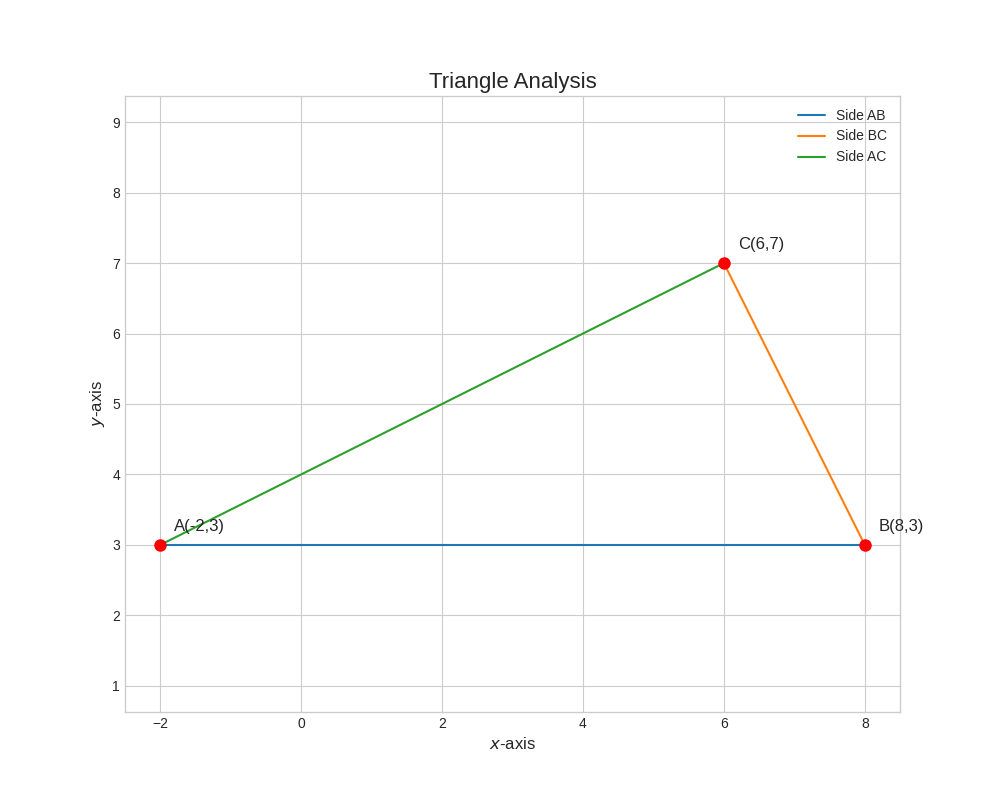
\includegraphics[width=0.7\columnwidth]{figs/Figure_1.png}
    \label{fig:placeholder}
\end{figure}
\end{frame}
\end{document}
